\citeauthor{Drucker2015} describe a tool which makes use of so called unit visualizations. This type of visualization is best described as using one complete row of a dataset and representing it as a unit. Advantages of using units are described in the following list \iacite{Drucker2015}:
\begin{itemize}
\item \textbf{The forest and the trees:} when using a visualization based on aggregation of data, it is possible to hide outlying data or have outlying data influence the representation \iacite{Drucker2015}. However, unit visualizations maintain a one-to-one correspondence between rows in a dataset with the represenation. While classical bar charts only show one static bar for each aggregated attribute, unit visualizations show the dynamic units building that bar. Therefore, a bar for a bar chart made in a unit visualization is not a single, static shape. It is a dynamically created bar with shapes representing each unit individually and thus showing the trees yielding the forest instead of showing only the forest.

\item \textbf{Semantic constancy:} the connection between a row and a unit is maintained throughout all changes. Thus, changing visual attributes or switching from one visualization to another, does not break that bond.

\item \textbf{Direct interaction:} when using the concept of unit visualizations, it is fairly easy to show additional information of each unit by providing for example tooltips. Even when using multiple views, the concept of linking and brushing (see chapter \ref{s:linking-brushing} on page \pageref{s:linking-brushing} fore more information) can be accomplished by highlighting the selected units in every view. Furthermore, if some kind of aggregated visualization is implemented with this concept, the units can still be highlighted because they are still visible.

\item \textbf{Animation:} because of the semantic constancy, it is possible to animate smoothly between different visualizations. Transitions only update the position of every unit since they are all present.

\end{itemize}

Albeit showing a lot of advantages, the concept of unit visualizations show some weaknesses:

\begin{itemize}
\item Using a lot of units, for example, in a bar can lead to visual clutter compared to a single, static aggregated one.

\item Accessing the information of the aggregation needs more calculation in a unit visualization because each unit already represents its row and still needs to know its particular group for aggregation. First, this group needs to be calculated and second, some attributes e.g. count or sum needs to be shown in the visualization.

\item Scaling is the main weakness of this type of visualizations. Aggregate visualizations can potentially use a much larger dataset, compared to unit visualizations. Scaling does not only include the amount of data used, it also includes the hardware accessible. Displaying thousands of items and animating them requires more operation power than calculating an aggregation and drawing a rectangle on a fixed position.

\end{itemize}

\begin{figure}[!htb]
\centering
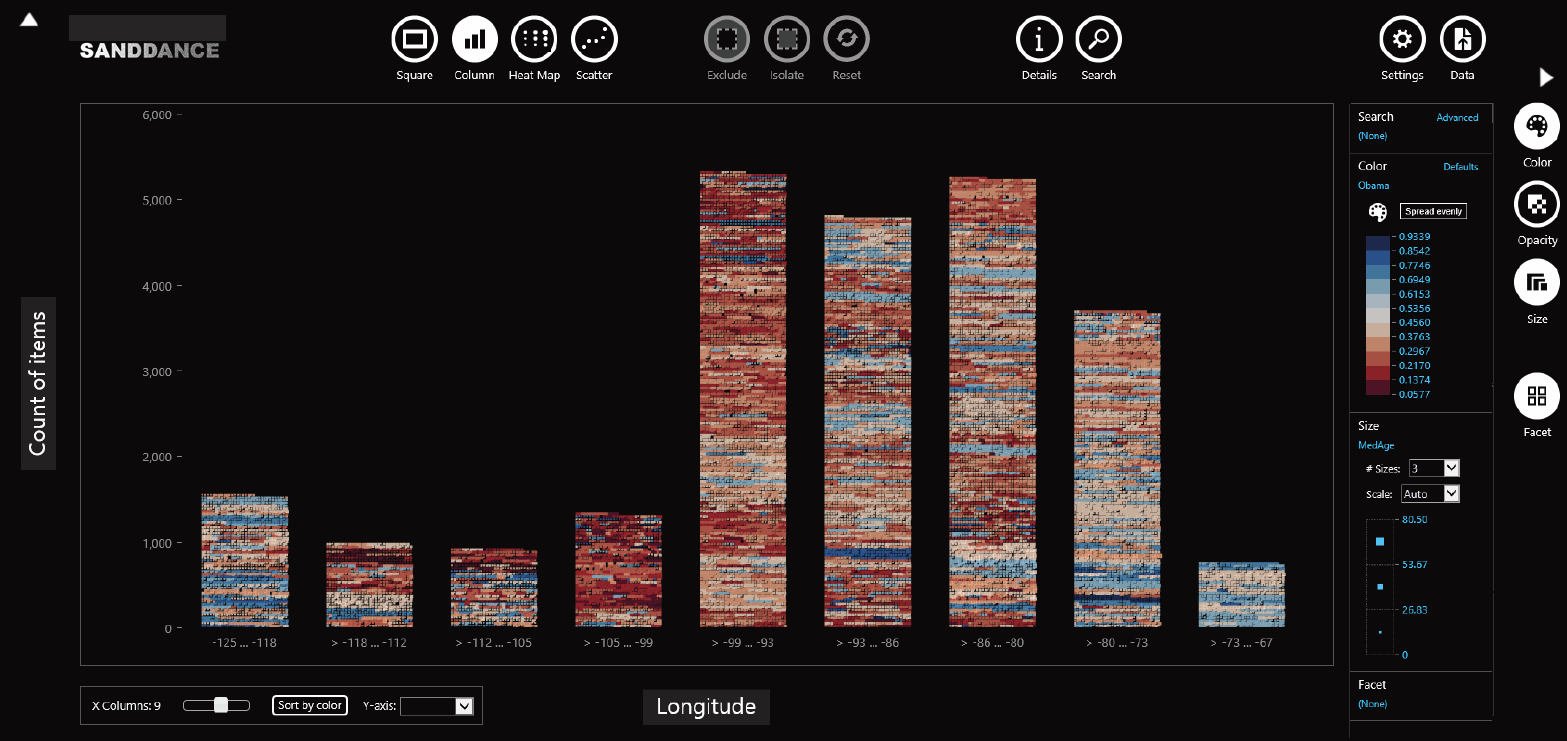
\includegraphics[width=0.8\textwidth,keepaspectratio]{images/methods/related/sanddance.png}
\caption[
    Concept of SandDance \iacite{Drucker2015}.
]{SandDance}
\label{fig:sanddance}
\end{figure}

Figure \ref{fig:sanddance} on page \pageref{fig:sanddance} shows the prototype. It allows to manually change visual channels to the right and change visual appearance e.g. changing the type of visualization at the top left. According to the analysis framework, SandDance uses static tables as input data only. \citeauthor{Drucker2015} states, that the tool was built to explore the benefits of using unit visualizations. Therefore it has no real use case to analyse, because it was used to show a completly different type of visualization without considering user benefit. However, one could say that the tool can be used to consume information and maybe discover new knowledge if using non-preexistent datasets.
SandDance can be still analysed when looking at how they implemented the visualization idiom: they freely allow users to encode attributes, even suggesting appropriate values automatically. Manipulation is implemented with a possible change in visual appearance and selection of shown data. The selection can further be filtered in different ways by either isolating or excluding data based on the given criteria.